\documentclass{article}

\usepackage{fullpage}
\usepackage{nopageno}
\usepackage{amsmath}
\usepackage{amsfonts}
\usepackage{graphicx}
\usepackage{algorithmic}
\usepackage{xcolor}
\usepackage{framed}

\definecolor{dark_red}{rgb}{0.5,0.0,0.0}

\newcommand{\abs}[1]{\left|#1\right|}
\newcommand{\atan}{\text{atan}}
\newcommand{\rowxyvec}[2]{\left\langle #1, #2 \right\rangle}
\newcommand{\rowvec}[3]{\left\langle #1, #2, #3 \right\rangle}
\newcommand{\colxyvec}[2]{\begin{bmatrix} #1 \\ #2 \end{bmatrix}}
\newcommand{\colvec}[3]{\begin{bmatrix} #1 \\ #2 \\ #3 \end{bmatrix}}
\newcommand{\at}[1]{\left. #1 \right|}
\newcommand{\diff}[2]{\frac{d #1}{d #2}}
\newcommand{\partdiff}[2]{\frac{\partial #1}{\partial #2}}
\newcommand{\mvec}[1]{\overrightarrow{\mathbf{#1}}}
\newcommand{\pvec}[1]{\overrightarrow{#1}}
\newcommand{\dr}[1]{\textcolor{dark_red}{#1}}


\title{Theorems related to Vector Calculus}
\date{}

\begin{document}

\maketitle


%%%%%%%%%%%%%%%%%%%%%%%%%% Question 1
\section*{Question 1:}

\subsection*{part 1a:}

Evaluate the scalar line integral: 

\[\int_C (6x^2 + 4y)ds \quad\text{where}\quad \mathbf{r}_C(t) = \colxyvec{3t + 2}{-t + 3} \;\text{and}\; t \in [-1,1]\]

\vspace{5mm}
\dr{\textbf{Solution:}}

\dr{\begin{align*}
\int_C (6x^2 + 4y)ds = & \int_{t=-1}^1 (6x_C(t)^2 + 4y_C(t))\abs{\frac{d\mathbf{r}_C}{dt}}dt \\
= & \int_{t=-1}^1 (6(3t+2)^2 + 4(-t+3))\abs{\colxyvec{3}{-1}}dt \\
= & \int_{t=-1}^1 ((54t^2 + 72t + 24) + (-4t+12))\sqrt{10} \cdot dt \\
= & \int_{t=-1}^1 (54t^2 + 68t + 36)\sqrt{10} \cdot dt \\
= & \at{(18t^3 + 34t^2 + 36t)\sqrt{10}}_{t=-1}^1 \\
= & (18 + 34 + 36)\sqrt{10} - (-18 + 34 - 36)\sqrt{10} \\
= & 88\sqrt{10} - (-20)\sqrt{10} 
= 108\sqrt{10}
\end{align*}}



\subsection*{part 1b:}

Evaluate the scalar line integral: 

\[\int_C (x^2 + 2y)ds \quad\text{where}\quad \mathbf{r}_C(t) = \colxyvec{1 - 2t}{2 - t} \;\text{and}\; t \in [0,3]\]

\vspace{5mm}
\dr{\textbf{Solution:}}

\dr{\begin{align*}
\int_C (x^2 + 2y)ds = & \int_{t=0}^3 (x_C(t)^2 + 2y_C(t))\abs{\frac{d\mathbf{r}_C}{dt}}dt \\
= & \int_{t=0}^3 ((1-2t)^2 + 2(2-t))\abs{\colxyvec{-2}{-1}}dt \\
= & \int_{t=0}^3 ((4t^2 - 4t + 1) + (-2t + 4))\sqrt{5} \cdot dt \\
= & \int_{t=0}^3 (4t^2 - 6t + 5)\sqrt{5} \cdot dt \\
= & \at{(\frac{4}{3}t^3 - 3t^2 + 5t)\sqrt{5}}_{t=0}^3 \\
= & (36 - 27 + 15)\sqrt{5} - 0 
= 24\sqrt{5}
\end{align*}}



\subsection*{part 1c:}

Evaluate the scalar line integral: 

\[\int_C 2x \cdot \sin(y) \cdot ds \quad\text{where}\quad \mathbf{r}_C(t) = \colxyvec{\cos(t)}{t} \;\text{and}\; t \in [0,\pi/2]\]

\vspace{5mm}
\dr{\textbf{Solution:}}

\dr{\begin{align*}
\int_C 2x \cdot \sin(y) \cdot ds = & \int_{t=0}^{\pi/2} 2x_C(t) \cdot \sin(y_C(t))\abs{\frac{d\mathbf{r}_C}{dt}}dt \\ 
= & \int_{t=0}^{\pi/2} 2\cos(t)\sin(t)\abs{\colxyvec{-\sin(t)}{1}}dt \\
= & \int_{t=0}^{\pi/2} 2\cos(t)\sin(t)\sqrt{\sin^2(t) + 1}dt \\
= & \at{\frac{2}{3}(\sin^2(t) + 1)^{3/2}}_{t=0}^{\pi/2} 
= \frac{2}{3}(2^{3/2} - 1)
\end{align*}}



%%%%%%%%%%%%%%%%%%%%%%%%%% Question 2
\section*{Question 2:}

\subsection*{part 2a:}

Evaluate the vector line integral: 

\[\int_C \colxyvec{-6x}{4y} \cdot d\mathbf{r} \quad\text{where}\quad \mathbf{r}_C(t) = \colxyvec{t^2}{1/t} \;\text{and}\; t \in [1,2]\]

\vspace{5mm}
\dr{\textbf{Solution:}}

\dr{\begin{align*}
\int_C \colxyvec{-6x}{4y} \cdot d\mathbf{r} = & \int_{t=1}^2 \colxyvec{-6x_C(t)}{4y_C(t)} \cdot \frac{d\mathbf{r}_C}{dt}dt 
= \int_{t=1}^2 \colxyvec{-6t^2}{4/t} \cdot \colxyvec{2t}{-1/t^2}dt \\
= & \int_{t=1}^2 (-12t^3 - \frac{4}{t^3})dt 
= \at{(-3t^4 + \frac{2}{t^2})}_{t=1}^2 \\
= & (-48 + \frac{1}{2}) - (-3 + 2) 
= -47 + \frac{1}{2} = -\frac{93}{2}
\end{align*}}



\subsection*{part 2b:}

Evaluate the vector line integral: 

\[\int_C \colxyvec{y}{x} \cdot d\mathbf{r} \quad\text{where}\quad \mathbf{r}_C(t) = \colxyvec{t^3}{t^4} \;\text{and}\; t \in [0,2]\]

\vspace{5mm}
\dr{\textbf{Solution:}}

\dr{\begin{align*}
\int_C \colxyvec{y}{x} \cdot d\mathbf{r} = & \int_{t=0}^2 \colxyvec{y_C(t)}{x_C(t)} \cdot \frac{d\mathbf{r}_C}{dt}dt 
= \int_{t=0}^2 \colxyvec{t^4}{t^3} \cdot \colxyvec{3t^2}{4t^3}dt 
= \int_{t=0}^2 7t^6 dt 
= \at{t^7}_{t=0}^2 
= 128
\end{align*}}




\subsection*{part 2c:}

Evaluate the vector line integral: 

\[\int_C \colvec{2x}{y^2}{-z} \cdot d\mathbf{r} \quad\text{where}\quad \mathbf{r}_C(t) = \colvec{-t^2}{t+4}{3t+2} \;\text{and}\; t \in [-1,1]\]

\vspace{5mm}
\dr{\textbf{Solution:}}

\dr{\begin{align*}
\int_C \colvec{2x}{y^2}{-z} \cdot d\mathbf{r} = & \int_{t=-1}^1 \colvec{2x_C(t)}{y_C(t)^2}{-z_C(t)} \cdot \frac{d\mathbf{r}_C}{dt}dt 
= \int_{t=-1}^1 \colvec{-2t^2}{t^2 + 8t + 16}{-3t - 2} \cdot \colvec{-2t}{1}{3}dt \\
= & \int_{t=-1}^1 (4t^3 + (t^2 + 8t + 16) + (-9t - 6))dt 
= \int_{t=-1}^1 (4t^3 + t^2 - t + 10)dt \\
= & \at{(t^4 + \frac{1}{3}t^3 - \frac{1}{2}t^2 + 10t)}_{t=-1}^1 
= (1 + \frac{1}{3} - \frac{1}{2} + 10) - (1 - \frac{1}{3} - \frac{1}{2} - 10) \\
= & \frac{66 + 2 - 3}{6} - \frac{-54 - 2 - 3}{6} 
= \frac{65}{6} + \frac{59}{6} 
= \frac{124}{6} 
= \frac{62}{3}
\end{align*}}




%%%%%%%%%%%%%%%%%%%%%%%%%% Question 3
\section*{Question 3:}

%%%%%%%%%%%%%%%%%%%%%%%%% Question 3A
\subsection*{part 3a:}

Is the vector field \(\mathbf{F}(x,y,z) = \colvec{y^2\sin(z)}{2xy\sin(z)}{xy^2\cos(z)}\) conservative? If yes, use the {\bf gradient theorem} to evaluate the vector line integral:

\[\int_C \colvec{y^2\sin(z)}{2xy\sin(z)}{xy^2\cos(z)} \cdot d\mathbf{r} \quad\text{where}\quad \mathbf{r}_\text{initial} = \colvec{0}{0}{0} \;\text{and}\; \mathbf{r}_\text{final} = \colvec{1}{1}{\pi/2}\] 

%%%%%%%%%%%%%%% Solution 3a
\vspace{5mm}
\dr{\textbf{Solution:}}

\dr{The curl (circulation density) of \(\mathbf{F}(x,y,z) = \colvec{F_x(x,y,z)}{F_y(x,y,z)}{F_z(x,y,z)} = \colvec{y^2\sin(z)}{2xy\sin(z)}{xy^2\cos(z)}\) is: 
\begin{align*}
\nabla \times \mathbf{F} = \colvec{\partial F_z/\partial y - \partial F_y/\partial z}{\partial F_x/\partial z - \partial F_z/\partial x}{\partial F_y/\partial x - \partial F_x/\partial y} = & \colvec{2xy\cos(z) - 2xy\cos(z)}{y^2\cos(z) - y^2\cos(z)}{2y\sin(z) - 2y\sin(z)} = \colvec{0}{0}{0} = \mathbf{0}
\end{align*}}

\dr{Since the curl is \(\mathbf{0}\) everywhere \(\mathbf{F}(x,y,z)\) is conservative, and the vector line integral \(\int_C \mathbf{F}(x,y,z) \cdot d\mathbf{r}\) depends only on the endpoints of \(C\), and not on any of the interior points of \(C\). Now to find a function \(f(x,y,z)\) where \(\nabla f = \colvec{y^2\sin(z)}{2xy\sin(z)}{xy^2\cos(z)}\):
\begin{align*}
f(x,y,z) = & f_0 + \int_{x_1 = 0}^x F_x(x_1,0,0)dx_1 + \int_{y_1 = 0}^y F_y(x,y_1,0)dy_1 + \int_{z_1 = 0}^z F_z(x,y,z_1)dz_1 \\
= & f_0 + \int_{x_1 = 0}^x 0dx_1 + \int_{y_1 = 0}^y 0dy_1 + \int_{z_1 = 0}^z xy^2\cos(z_1) dz_1 \\
= & f_0 + \at{xy^2\sin(z_1)}_{z_1 = 0}^z 
= f_0 + xy^2\sin(z)
\end{align*}}

\dr{Using the gradient theorem,
\begin{align*}
\int_C \colvec{y^2\sin(z)}{2xy\sin(z)}{xy^2\cos(z)} \cdot d\mathbf{r} = & \int_C (\nabla f) \cdot d\mathbf{r} 
= f(1,1,\pi/2) - f(0,0,0) 
= (f_0 + 1) - f_0 
= 1
\end{align*}}



%%%%%%%%%%%%%%%%%%%%%%%%% Question 3B
\subsection*{part 3b:}

Is the vector field \(\mathbf{F}(x,y,z) = \colvec{xy}{xy}{z}\) conservative? If yes, use the {\bf gradient theorem} to evaluate the vector line integral:

\[\int_C \colvec{xy}{xy}{z} \cdot d\mathbf{r} \quad\text{where}\quad \mathbf{r}_\text{initial} = \colvec{0}{0}{0} \;\text{and}\; \mathbf{r}_\text{final} = \colvec{1}{1}{1}\] 

%%%%%%%%%%%%%%% Solution 3b
\vspace{5mm}
\dr{\textbf{Solution:}}

\dr{The curl (circulation density) of \(\mathbf{F}(x,y,z) = \colvec{F_x(x,y,z)}{F_y(x,y,z)}{F_z(x,y,z)} = \colvec{xy}{xy}{z}\) is: 
\begin{align*}
\nabla \times \mathbf{F} = \colvec{\partial F_z/\partial y - \partial F_y/\partial z}{\partial F_x/\partial z - \partial F_z/\partial x}{\partial F_y/\partial x - \partial F_x/\partial y} = & \colvec{0 - 0}{0 - 0}{y - x} = \colvec{0}{0}{y - x}
\end{align*}}

\dr{Since the curl is not \(\mathbf{0}\) everywhere \(\mathbf{F}(x,y,z)\) is {\bf not} conservative, and the vector line integral \\ \(\int_C \mathbf{F}(x,y,z) \cdot d\mathbf{r}\) depends on the interior points of \(C\).}




%%%%%%%%%%%%%%%%%%%%%%%%%% Question 4
\section*{Question 4:}

%%%%%%%%%%%%%%%%%%%%%%%%% Question 4A
\subsection*{part 4a:}

\begin{tabular}{cc}
\parbox{0.6\textwidth}{ 
The region \(\sigma\) on the right is 
\[\sigma = \{(x,y) | 0 \leq x \leq 6 \;\text{and}\; 0 \leq y \leq 3 - (1/2)x\}\]
Use Green's theorem to compute the loop integral
\[\int_{\partial\sigma} \colxyvec{3x-5y}{x-2y} \cdot d\mathbf{r}\]
where \(\partial\sigma\) is the counterclockwise oriented boundary of \(\sigma\).
} & \parbox{0.4\textwidth}{
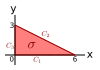
\includegraphics[width = 0.4\textwidth]{Test_bench_part_4x_images/Test_bench_part_4x_image_1}
}
\end{tabular}
Next, compute each of \(\int_{C_1} \colxyvec{3x-5y}{x-2y} \cdot d\mathbf{r}\); \(\int_{C_2} \colxyvec{3x-5y}{x-2y} \cdot d\mathbf{r}\); and \(\int_{C_3} \colxyvec{3x-5y}{x-2y} \cdot d\mathbf{r}\) and show that 
\[\int_{\partial\sigma} \colxyvec{3x-5y}{x-2y} \cdot d\mathbf{r} = \int_{C_1} \colxyvec{3x-5y}{x-2y} \cdot d\mathbf{r} + \int_{C_2} \colxyvec{3x-5y}{x-2y} \cdot d\mathbf{r} + \int_{C_3} \colxyvec{3x-5y}{x-2y} \cdot d\mathbf{r}\]  

%%%%%%%%%%%%%%% Solution 4a
\vspace{5mm}
\dr{\textbf{Solution:}}

\dr{Using Green's theorem gives:
\begin{align*} 
\int_{\partial\sigma} \colxyvec{3x-5y}{x-2y} \cdot d\mathbf{r} = & \iint_{\sigma} (\frac{\partial}{\partial x}(x - 2y) - \frac{\partial}{\partial y}(3x - 5y))dA 
= \iint_{\sigma} (1 - (-5))dA 
= \iint_{\sigma} 6dA \\
= & \int_{x=0}^6 \int_{y=0}^{3 - (1/2)x} 6 dydx 
= \int_{x=0}^6 \at{6y}_{y=0}^{3 - (1/2)x} dx  
= \int_{x=0}^6 (18 - 3x)dx \\
= & \at{(18x - \frac{3}{2}x^2)}_{x=0}^6   
= (108 - 54) - 0 
= 54
\end{align*}}  

\dr{One possible parameterization of \(C_1\) is \(\mathbf{r}_{C_1}(t) = \colxyvec{t}{0} \;\text{and}\; t \in [0,6]\) so
\begin{align*}
\int_{C_1} \colxyvec{3x-5y}{x-2y} \cdot d\mathbf{r} = & \int_{t=0}^6 \colxyvec{3x_{C_1}(t) - 5y_{C_1}(t)}{x_{C_1}(t) - 2y_{C_1}(t)} \cdot \frac{d\mathbf{r}_{C_1}}{dt}dt \\
= & \int_{t=0}^6 \colxyvec{3t}{t} \cdot \colxyvec{1}{0}dt 
= \int_{t=0}^6 3t dt 
= \at{\frac{3}{2}t^2}_{t=0}^6 
= 54
\end{align*}}

\dr{One possible parameterization of \(C_2\) is \(\mathbf{r}_{C_2}(t) = \colxyvec{6-t}{3 - (1/2)(6 - t)} = \colxyvec{6-t}{(1/2)t} \;\text{and}\; t \in [0,6]\) so
\begin{align*}
\int_{C_2} \colxyvec{3x-5y}{x-2y} \cdot d\mathbf{r} = & \int_{t=0}^6 \colxyvec{3x_{C_2}(t) - 5y_{C_2}(t)}{x_{C_2}(t) - 2y_{C_2}(t)} \cdot \frac{d\mathbf{r}_{C_2}}{dt}dt \\
= & \int_{t=0}^6 \colxyvec{(18 - 3t) - (5/2)t}{(6 - t) - t} \cdot \colxyvec{-1}{1/2}dt 
= \int_{t=0}^6 \colxyvec{18 - (11/2)t}{6 - 2t} \cdot \colxyvec{-1}{1/2}dt \\
= & \int_{t=0}^6 (-15 + (9/2)t)dt 
= \at{(-15t + (9/4)t^2)}_{t=0}^6 \\
= & (-90 + 81) - 0 
= -9 
\end{align*}}

\dr{One possible parameterization of \(C_3\) is \(\mathbf{r}_{C_3}(t) = \colxyvec{0}{3 - t} \;\text{and}\; t \in [0,3]\) so
\begin{align*}
\int_{C_3} \colxyvec{3x-5y}{x-2y} \cdot d\mathbf{r} = & \int_{t=0}^3 \colxyvec{3x_{C_3}(t) - 5y_{C_3}(t)}{x_{C_2}(t) - 2y_{C_3}(t)} \cdot \frac{d\mathbf{r}_{C_3}}{dt}dt \\
= & \int_{t=0}^3 \colxyvec{5t - 15}{2t - 6} \cdot \colxyvec{0}{-1}dt 
= \int_{t=0}^3 (6 - 2t)dt 
= \at{(6t - t^2)}_{t=0}^3 \\
= & (18 - 9) - 0 
= 9 
\end{align*}}

\dr{Therefore: \[\int_{C_1} \colxyvec{3x-5y}{x-2y} \cdot d\mathbf{r} + \int_{C_2} \colxyvec{3x-5y}{x-2y} \cdot d\mathbf{r} + \int_{C_3} \colxyvec{3x-5y}{x-2y} \cdot d\mathbf{r} = 54 + (-9) + 9 = 54 = \int_{\partial\sigma} \colxyvec{3x-5y}{x-2y} \cdot d\mathbf{r}\]}



%%%%%%%%%%%%%%%%%%%%%%%%%% Question 4B
\subsection*{part 4b:}

\begin{tabular}{cc}
\parbox{0.6\textwidth}{ 
The region \(\sigma\) on the right is 
\[\sigma = \{(x,y) | 0 \leq x \leq 1 \;\text{and}\; x^3 \leq y \leq x\}\]
Use Green's theorem to compute the loop integral
\[\int_{\partial\sigma} \colxyvec{2xy}{x+y} \cdot d\mathbf{r}\]
where \(\partial\sigma\) is the counterclockwise oriented boundary of \(\sigma\).
} & \parbox{0.4\textwidth}{
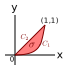
\includegraphics[width = 0.4\textwidth]{Test_bench_part_4x_images/Test_bench_part_4x_image_2}
}
\end{tabular}
Next, compute each of \(\int_{C_1} \colxyvec{2xy}{x+y} \cdot d\mathbf{r}\); and \(\int_{C_2} \colxyvec{2xy}{x+y} \cdot d\mathbf{r}\) and show that 
\[\int_{\partial\sigma} \colxyvec{2xy}{x+y} \cdot d\mathbf{r} = \int_{C_1} \colxyvec{2xy}{x+y} \cdot d\mathbf{r} + \int_{C_2} \colxyvec{2xy}{x+y} \cdot d\mathbf{r}\]  

%%%%%%%%%%%%%%% Solution 4b
\vspace{5mm}
\dr{\textbf{Solution:}}

\dr{Using Green's theorem gives:
\begin{align*} 
\int_{\partial\sigma} \colxyvec{2xy}{x+y} \cdot d\mathbf{r} = & \iint_{\sigma} (\frac{\partial}{\partial x}(x+y) - \frac{\partial}{\partial y}(2xy))dA \\
= & \iint_{\sigma} (1 - 2x)dA 
= \int_{x = 0}^1 \int_{y = x^3}^x (1 - 2x)dydx \\
= & \int_{x = 0}^1 \at{(1 - 2x)y}_{y = x^3}^x dx 
= \int_{x = 0}^1 ((-2x^2 + x) - (-2x^4 + x^3)) dx \\
= & \int_{x = 0}^1 (2x^4 - x^3 - 2x^2 + x) dx 
= \at{(\frac{2}{5}x^5 - \frac{1}{4}x^4 - \frac{2}{3}x^3 + \frac{1}{2}x^2)}_{x = 0}^1 \\
= & (\frac{2}{5} - \frac{1}{4} - \frac{2}{3} + \frac{1}{2}) - 0 
= \frac{24 - 15 - 40 + 30}{60} 
= \frac{9 - 10}{60} 
= -\frac{1}{60}
\end{align*}}  

\dr{One possible parameterization of \(C_1\) is \(\mathbf{r}_{C_1}(t) = \colxyvec{t}{t^3} \;\text{and}\; t \in [0,1]\) so
\begin{align*}
\int_{C_1} \colxyvec{2xy}{x+y} \cdot d\mathbf{r} = & \int_{t=0}^1 \colxyvec{2x_{C_1}(t)y_{C_1}(t)}{x_{C_1}(t)+y_{C_1}(t)} \cdot \frac{d\mathbf{r}_{C_1}}{dt}dt \\
= & \int_{t=0}^1 \colxyvec{2t^4}{t + t^3} \cdot \colxyvec{1}{3t^2}dt 
= \int_{t=0}^1 (3t^5 + 2t^4 + 3t^3)dt \\
= & \at{(\frac{1}{2}t^6 + \frac{2}{5}t^5 + \frac{3}{4}t^4)}_{t=0}^1 
= (\frac{1}{2} + \frac{2}{5} + \frac{3}{4}) - 0 \\
= & \frac{10 + 8 + 15}{20} 
= \frac{33}{20}
\end{align*}}

\dr{One possible parameterization of \(C_2\) is \(\mathbf{r}_{C_2}(t) = \colxyvec{1-t}{1-t} \;\text{and}\; t \in [0,1]\) so
\begin{align*}
\int_{C_2} \colxyvec{2xy}{x+y} \cdot d\mathbf{r} = & \int_{t=0}^1 \colxyvec{2x_{C_2}(t)y_{C_2}(t)}{x_{C_2}(t)+y_{C_2}(t)} \cdot \frac{d\mathbf{r}_{C_2}}{dt}dt \\ 
= & \int_{t=0}^1 \colxyvec{2(1-t)^2}{(1-t) + (1-t)} \cdot \colxyvec{-1}{-1}dt 
= \int_{t=0}^1 \colxyvec{2t^2 - 4t + 2}{-2t + 2} \cdot \colxyvec{-1}{-1}dt \\
= & \int_{t=0}^1 (-2t^2 + 6t - 4)dt 
= \at{(-\frac{2}{3}t^3 + 3t^2 - 4t)}_{t=0}^1 \\
= & (-\frac{2}{3} + 3 - 4) - 0 
= -\frac{5}{3}
\end{align*}}

\dr{Therefore: \[\int_{C_1} \colxyvec{2xy}{x+y} \cdot d\mathbf{r} + \int_{C_2} \colxyvec{2xy}{x+y} \cdot d\mathbf{r} = \frac{33}{20} + -\frac{5}{3} = -\frac{1}{60} = \int_{\partial\sigma} \colxyvec{2xy}{x+y} \cdot d\mathbf{r}\]}



%%%%%%%%%%%%%%%%%%%%%%%%%% Question 4C
\subsection*{part 4c:}

\begin{tabular}{cc}
\parbox{0.6\textwidth}{ 
The region \(\sigma\) on the right is 
\[\sigma = \{(x,y) | -4 \leq x \leq 0 \;\text{and}\; 0 \leq y \leq 2 + (1/2)x\}\]
Use Green's theorem to compute the loop integral
\[\int_{\partial\sigma} \colxyvec{x+2y}{5x+y} \cdot d\mathbf{r}\]
where \(\partial\sigma\) is the counterclockwise oriented boundary of \(\sigma\).
} & \parbox{0.4\textwidth}{
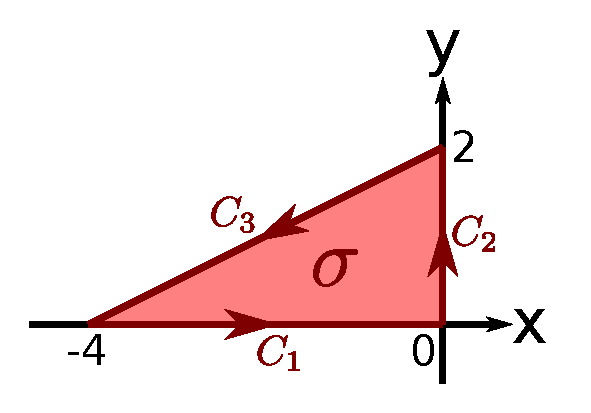
\includegraphics[width = 0.4\textwidth]{Test_bench_part_4x_images/Test_bench_part_4x_image_3}
}
\end{tabular}
Next, compute each of \(\int_{C_1} \colxyvec{x+2y}{5x+y} \cdot d\mathbf{r}\); \(\int_{C_2} \colxyvec{x+2y}{5x+y} \cdot d\mathbf{r}\); and \(\int_{C_3} \colxyvec{x+2y}{5x+y} \cdot d\mathbf{r}\) and show that 
\[\int_{\partial\sigma} \colxyvec{x+2y}{5x+y} \cdot d\mathbf{r} = \int_{C_1} \colxyvec{x+2y}{5x+y} \cdot d\mathbf{r} + \int_{C_2} \colxyvec{x+2y}{5x+y} \cdot d\mathbf{r} + \int_{C_3} \colxyvec{x+2y}{5x+y} \cdot d\mathbf{r}\]  

%%%%%%%%%%%%%%% Solution 4c
\vspace{5mm}
\dr{\textbf{Solution:}}

\dr{Using Green's theorem gives:
\begin{align*} 
\int_{\partial\sigma} \colxyvec{x+2y}{5x+y} \cdot d\mathbf{r} = & \iint_{\sigma} (\frac{\partial}{\partial x}(5x+y) - \frac{\partial}{\partial y}(x+2y))dA 
= \iint_{\sigma} (5 - 2)dA
= \iint_{\sigma} 3dA \\
= & \int_{x = -4}^0 \int_{y=0}^{2 + (1/2)x} 3dydx 
= \int_{x = -4}^0 \at{3y}_{y=0}^{2 + (1/2)x}dx 
= \int_{x = -4}^0 (6 + (3/2)x)dx \\
= & \at{(6x + (3/4)x^2)}_{x = -4}^0 
= 0 - (-24 + 12) 
= 12
\end{align*}}  

\dr{One possible parameterization of \(C_1\) is \(\mathbf{r}_{C_1}(t) = \colxyvec{t}{0} \;\text{and}\; t \in [-4,0]\) so
\begin{align*}
\int_{C_1} \colxyvec{x+2y}{5x+y} \cdot d\mathbf{r} = & \int_{t=-4}^0 \colxyvec{x_{C_1}(t)+2y_{C_1}(t)}{5x_{C_1}(t)+y_{C_1}(t)} \cdot \frac{d\mathbf{r}_{C_1}}{dt}dt \\
= & \int_{t=-4}^0 \colxyvec{t}{5t} \cdot \colxyvec{1}{0}dt 
= \int_{t=-4}^0 t dt 
= \at{\frac{1}{2}t^2}_{t=-4}^0 
= -8
\end{align*}}

\dr{One possible parameterization of \(C_2\) is \(\mathbf{r}_{C_2}(t) = \colxyvec{0}{t} \;\text{and}\; t \in [0,2]\) so
\begin{align*}
\int_{C_2} \colxyvec{x+2y}{5x+y} \cdot d\mathbf{r} = & \int_{t=0}^2 \colxyvec{x_{C_2}(t)+2y_{C_2}(t)}{5x_{C_2}(t)+y_{C_2}(t)} \cdot \frac{d\mathbf{r}_{C_2}}{dt}dt \\ 
= & \int_{t=0}^2 \colxyvec{2t}{t} \cdot \colxyvec{0}{1}dt 
= \int_{t=0}^2 t dt  
= \at{\frac{1}{2}t^2}_{t=0}^2 
= 2
\end{align*}}

\dr{One possible parameterization of \(C_3\) is \(\mathbf{r}_{C_3}(t) = \colxyvec{-t}{2 - (1/2)t} \;\text{and}\; t \in [0,4]\) so
\begin{align*}
\int_{C_3} \colxyvec{x+2y}{5x+y} \cdot d\mathbf{r} = & \int_{t=0}^4 \colxyvec{x_{C_3}(t)+2y_{C_3}(t)}{5x_{C_3}(t)+y_{C_3}(t)} \cdot \frac{d\mathbf{r}_{C_3}}{dt}dt \\ 
= & \int_{t=0}^4 \colxyvec{-t + (4 - t)}{-5t + (2 - (1/2)t)} \cdot \colxyvec{-1}{-1/2}dt 
= \int_{t=0}^4 \colxyvec{-2t + 4}{-(11/2)t + 2} \cdot \colxyvec{-1}{-1/2}dt \\
= & \int_{t=0}^4 ((2t - 4) + ((11/4)t - 1))dt 
= \int_{t=0}^4 ((19/4)t - 5)dt 
= \at{((19/8)t^2 - 5t)}_{t=0}^4 \\
= & (38 - 20) - 0 
= 18 
\end{align*}}

\dr{Therefore: \[\int_{C_1} \colxyvec{x+2y}{5x+y} \cdot d\mathbf{r} + \int_{C_2} \colxyvec{x+2y}{5x+y} \cdot d\mathbf{r} + \int_{C_3} \colxyvec{x+2y}{5x+y} \cdot d\mathbf{r} = -8 + 2 + 18 = 12 = \int_{\partial\sigma} \colxyvec{x+2y}{5x+y} \cdot d\mathbf{r}\]}




%%%%%%%%%%%%%%%%%%%%%%%%%% Question 5 
\section*{Question 5:}

\begin{tabular}{cc}
\parbox{0.6\textwidth}{ 
The region \(\sigma\) on the right is 
\[\sigma = \{(x,y) | 0 \leq x \leq 1 \;\text{and}\; 0 \leq y \leq 1 - x^2\}\]
Use Gauss's divergence theorem to compute the flux integral
\[\int_{\partial\sigma} \colxyvec{x^2}{y} \cdot \colxyvec{dy}{-dx}\]
where \(\partial\sigma\) is the counterclockwise oriented boundary of \(\sigma\).
} & \parbox{0.4\textwidth}{
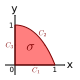
\includegraphics[width = 0.4\textwidth]{Test_bench_part_4x_images/Test_bench_part_4x_image_4}
}
\end{tabular}
Next, compute each of \(\int_{C_1} \colxyvec{x^2}{y} \cdot \colxyvec{dy}{-dx}\); \(\int_{C_2} \colxyvec{x^2}{y} \cdot \colxyvec{dy}{-dx}\); and \(\int_{C_3} \colxyvec{x^2}{y} \cdot \colxyvec{dy}{-dx}\) and show that 
\[\int_{\partial\sigma} \colxyvec{x^2}{y} \cdot \colxyvec{dy}{-dx} = \int_{C_1} \colxyvec{x^2}{y} \cdot \colxyvec{dy}{-dx} + \int_{C_2} \colxyvec{x^2}{y} \cdot \colxyvec{dy}{-dx}+ \int_{C_3} \colxyvec{x^2}{y} \cdot \colxyvec{dy}{-dx}\]  

%%%%%%%%%%%%%%% Solution 5
\vspace{5mm}
\dr{\textbf{Solution:}}

\dr{Using Gauss's divergence theorem gives:
\begin{align*}
\int_{\partial\sigma} \colxyvec{x^2}{y} \cdot \colxyvec{dy}{-dx} = & \iint_{\sigma} (\frac{\partial}{\partial x}(x^2) + \frac{\partial}{\partial y}(y))dA 
= \iint_{\sigma} (2x + 1)dA \\
= & \int_{x=0}^1 \int_{y=0}^{1-x^2} (2x+1)dydx 
= \int_{x=0}^1 \at{(2x+1)y}_{y=0}^{1-x^2}dx \\
= & \int_{x=0}^1 ((2x+1)(1-x^2) - 0)dx 
= \int_{x=0}^1 (-2x^3 - x^2 + 2x + 1)dx \\
= & \at{(-\frac{1}{2}x^4 - \frac{1}{3}x^3 + x^2 + x)}_{x=0}^1 
= (-\frac{1}{2} - \frac{1}{3} + 2) - 0 \\
= & \frac{-3 - 2 + 12}{6} 
= \frac{7}{6} 
\end{align*}}

\dr{One possible parameterization of \(C_1\) is \(\mathbf{r}_{C_1}(t) = \colxyvec{t}{0} \;\text{and}\; t \in [0,1]\) so
\begin{align*}
\int_{C_1} \colxyvec{x^2}{y} \cdot \colxyvec{dy}{-dx} = & \int_{C_1} \colxyvec{-y}{x^2} \cdot d\mathbf{r}
= \int_{t=0}^1 \colxyvec{-y_{C_1}(t)}{x_{C_1}(t)^2} \cdot \frac{d\mathbf{r}_{C_1}}{dt}dt \\
= & \int_{t=0}^1 \colxyvec{0}{t^2} \cdot \colxyvec{1}{0}dt 
= \int_{t=0}^1 0dt 
= 0 
\end{align*}}

\dr{One possible parameterization of \(C_2\) is \(\mathbf{r}_{C_2}(t) = \colxyvec{1-t}{1-(1-t)^2} = \colxyvec{-t + 1}{-t^2 + 2t} \;\text{and}\; t \in [0,1]\) so
\begin{align*}
\int_{C_2} \colxyvec{x^2}{y} \cdot \colxyvec{dy}{-dx} = & \int_{C_2} \colxyvec{-y}{x^2} \cdot d\mathbf{r}
= \int_{t=0}^1 \colxyvec{-y_{C_2}(t)}{x_{C_2}(t)^2} \cdot \frac{d\mathbf{r}_{C_2}}{dt}dt \\
= & \int_{t=0}^1 \colxyvec{t^2 - 2t}{(-t + 1)^2} \cdot \colxyvec{-1}{-2t + 2}dt 
= \int_{t=0}^1 \colxyvec{t^2 - 2t}{t^2 - 2t + 1} \cdot \colxyvec{-1}{-2t + 2}dt \\
= & \int_{t=0}^1 ((-t^2 + 2t) + (-2t^3 + 6t^2 - 6t + 2))dt 
= \int_{t=0}^1 (-2t^3 + 5t^2 - 4t + 2)dt \\
= & \at{(-\frac{1}{2}t^4 + \frac{5}{3}t^3 - 2t^2 + 2t)}_{t=0}^1 
= (-\frac{1}{2} + \frac{5}{3}) - 0 
= \frac{-3 + 10}{6}
= \frac{7}{6}
\end{align*}}

\dr{One possible parameterization of \(C_3\) is \(\mathbf{r}_{C_3}(t) = \colxyvec{0}{1 - t} \;\text{and}\; t \in [0,1]\) so
\begin{align*}
\int_{C_3} \colxyvec{x^2}{y} \cdot \colxyvec{dy}{-dx} = & \int_{C_3} \colxyvec{-y}{x^2} \cdot d\mathbf{r} 
= \int_{t=0}^1 \colxyvec{-y_{C_3}(t)}{x_{C_3}(t)^2} \cdot \frac{d\mathbf{r}_{C_3}}{dt}dt \\ 
= & \int_{t=0}^1 \colxyvec{t - 1}{0} \cdot \colxyvec{0}{-1}dt 
= \int_{t=0}^1 0dt
= 0 
\end{align*}}

\dr{Therefore: \[\int_{C_1} \colxyvec{x^2}{y} \cdot \colxyvec{dy}{-dx} + \int_{C_2} \colxyvec{x^2}{y} \cdot \colxyvec{dy}{-dx} + \int_{C_3} \colxyvec{x^2}{y} \cdot \colxyvec{dy}{-dx} = 0 + \frac{7}{6} + 0 = \frac{7}{6} = \int_{\partial\sigma} \colxyvec{x^2}{y} \cdot \colxyvec{dy}{-dx}\]}

\end{document}









